\documentclass[final]{article}


\usepackage{APS360}
\usepackage[utf8]{inputenc}
\usepackage[T1]{fontenc}
\usepackage{hyperref}
\usepackage{url}
\usepackage{booktabs}
\usepackage{amsfonts}
\usepackage{nicefrac}
\usepackage{microtype}
\usepackage{xcolor}
\usepackage{graphicx}
\usepackage{float}

\makeatletter
\renewcommand{\@notice}{}
\makeatother

\title{CNN Logo Era Classification from Logopedia}
\author{%
  Derek Lau \\
  1012104679, \texttt{derek.lau@mail.utoronto.ca}\\
  \url{https://github.com/derek750/APS360-Project}\\
  Colab: \url{https://colab.research.google.com/github/derek750/APS360-Project/blob/master/notebooks/progress_report.ipynb}
}

\begin{document}

\maketitle
\vspace{-0.55in}

\setlength{\parskip}{3.5pt}
\setlength{\abovecaptionskip}{4pt}

\section*{Brief Project Description}

This project predicts the \textbf{design decade} of a corporate logo from a single image.
\textbf{Input:} a $224\times224$ RGB logo (transparent assets composited onto white).
\textbf{Output:} one of $K$ decade classes (e.g., \texttt{1990} for the 1990s).
Labels reflect \emph{when} a mark was introduced, not brand identity, so one company can span multiple classes while unrelated brands sharing era-wide typography, color, and layout group together.
\textbf{Deep learning} is appropriate because these cues are high-dimensional spatial patterns that are hard to hand-engineer; a shallow CNN can learn layout and ornamentation beyond palette statistics.

Figure~\ref{fig:pipeline} summarizes the pipeline: scrape Logopedia histories, label by introduction decade with company-level splits, train a shallow CNN, and compare to a Palermo-style color baseline on the same held-out brands.

\begin{figure}[H]
  \centering
  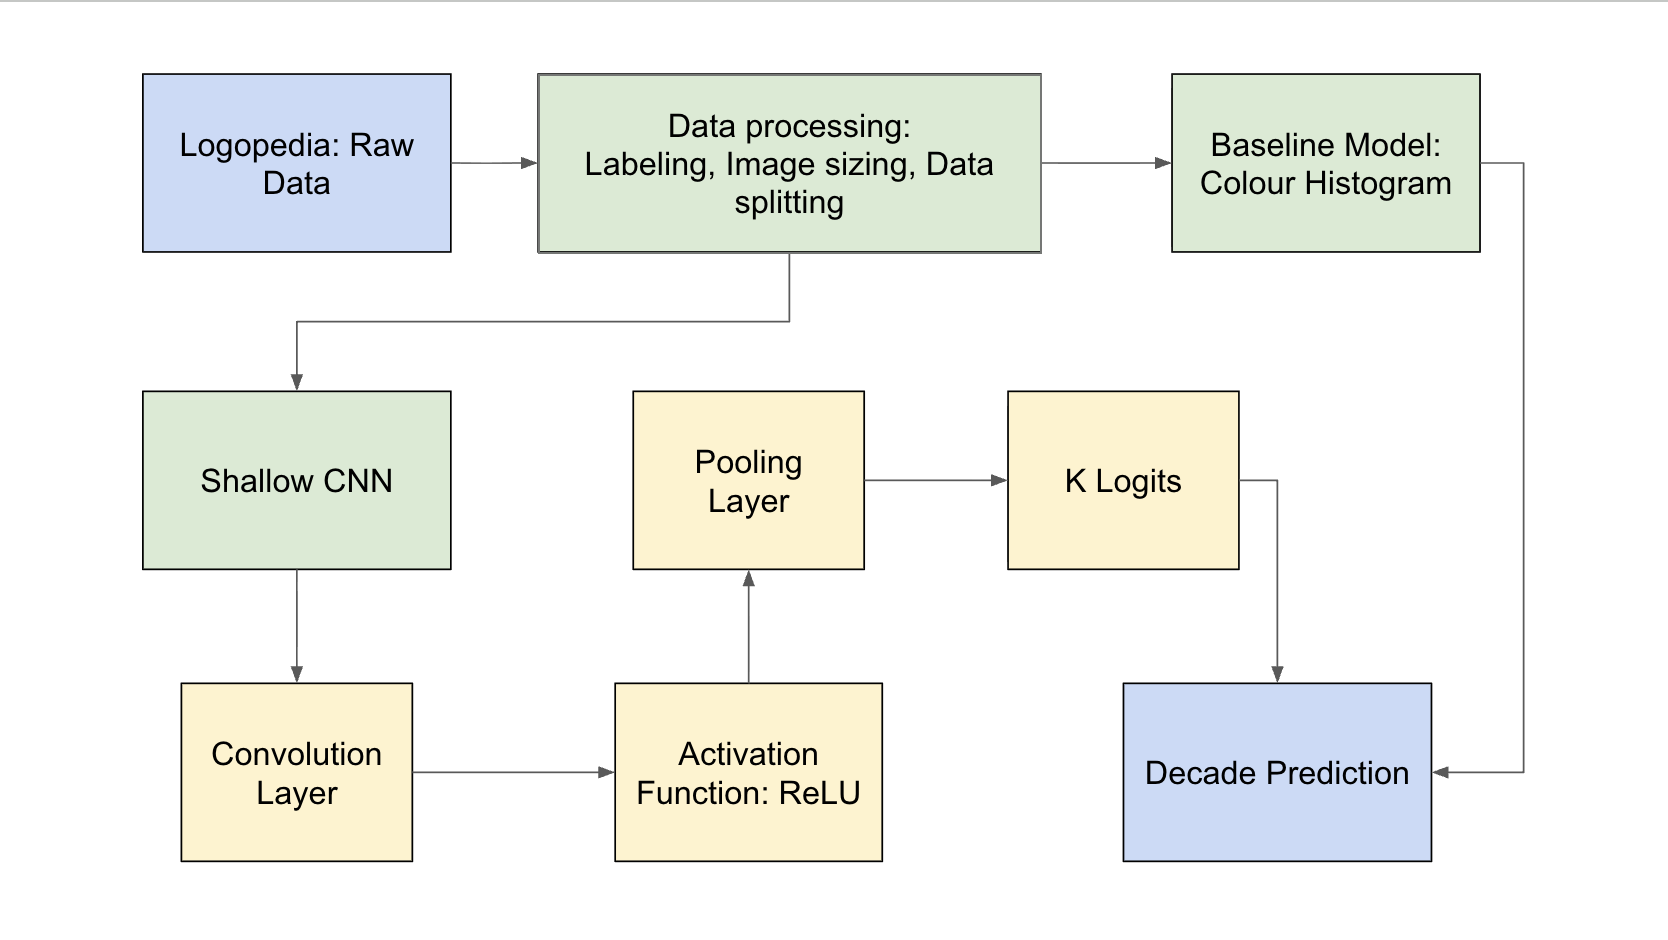
\includegraphics[width=0.74\linewidth,keepaspectratio]{figures/APS360_Pipeline.png}
  \caption{End-to-end pipeline. Both models share the same preprocessed images and company-level train/validation/test splits.}
  \label{fig:pipeline}
\end{figure}

\section*{Notable Contribution}

\textbf{Data Processing:}
I built a custom dataset from \textbf{Logopedia}\footnote{\url{https://logos.fandom.com}} via the MediaWiki Action API.
Companies were indexed from eight industry categories; for each page I parsed \texttt{ImageTOC} lines, section headers, and filenames with years, mapped start years to decades, resolved images with \texttt{prop=imageinfo}, composited transparent assets onto white, and resized to $224\times224$.
One logo per company-decade; splits are \textbf{by company} (70/15/15).

\begin{table}[H]
  \centering
  \caption{Cleaned dataset summary.}
  \label{tab:data}
  \small
  \begin{tabular}{@{}lr@{}}
    \toprule
    Statistic & Count \\
    \midrule
    Companies indexed / with logos & 250 / 236 \\
    Images; decade classes ($K$) & 428; 17 \\
    Train / val / test & 304 / 69 / 55 \\
    \bottomrule
  \end{tabular}
\end{table}

Figure~\ref{fig:data} shows class imbalance and sample logos.
\textbf{Final-test plan:} evaluate on companies scraped after this checkpoint.
\textbf{Challenges:} noisy crowd-sourced years; sparse early-decade examples.

\begin{figure}[H]
  \centering
  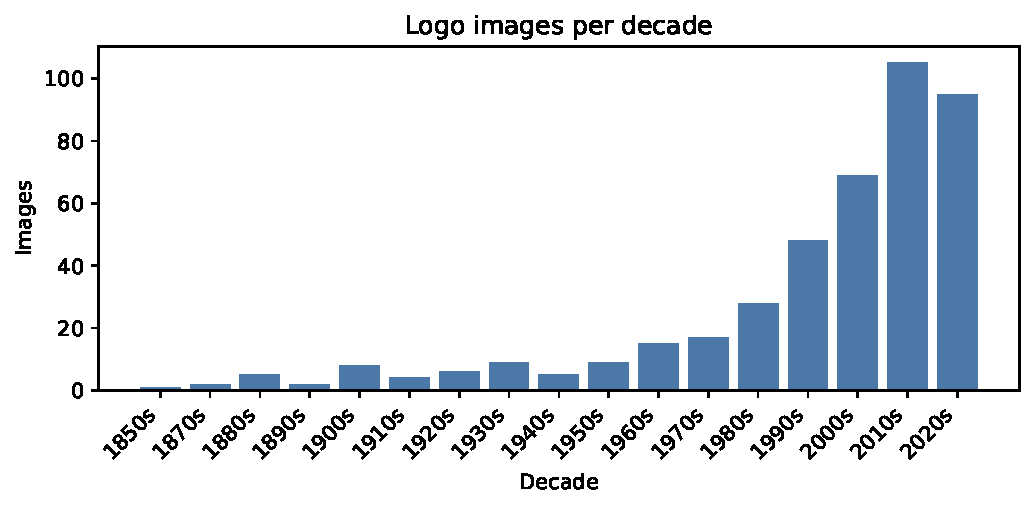
\includegraphics[width=0.42\linewidth]{figures/decade_distribution.pdf}\hfill
  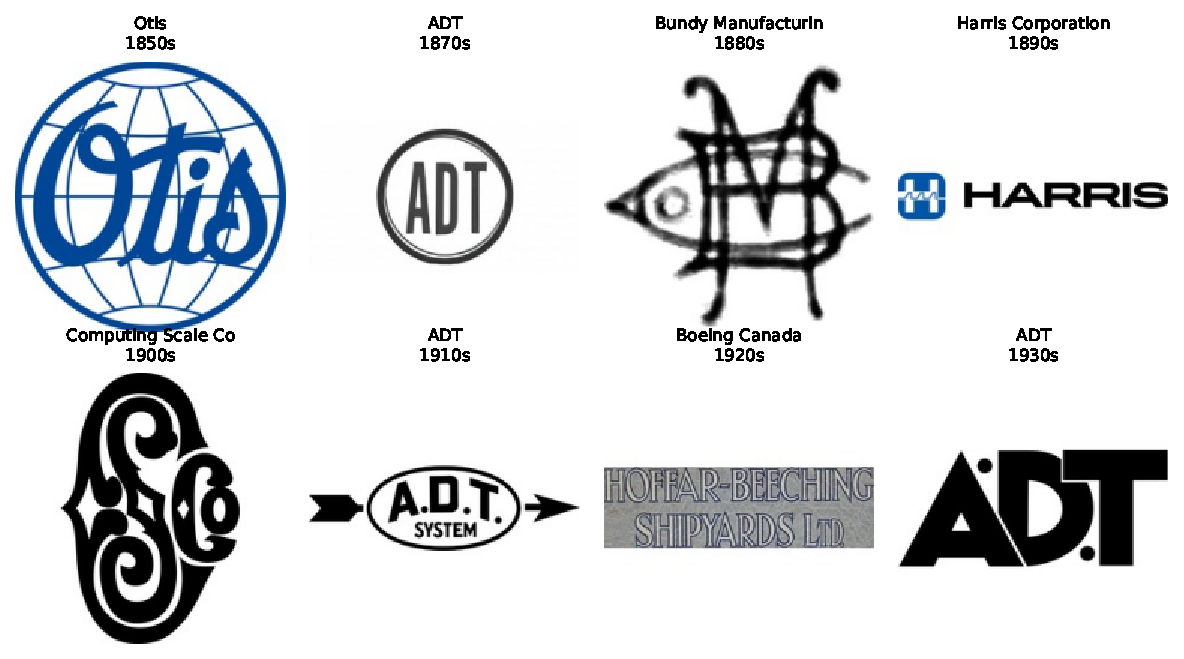
\includegraphics[width=0.52\linewidth]{figures/sample_logos.pdf}
  \caption{Left: images per decade. Right: labeled examples.}
  \label{fig:data}
\end{figure}

\textbf{Baseline Model:}
Per Palermo et al.~\cite{palermo2012dating}, I extracted RGB/HSV histograms (16 bins) and color moments per logo, standardized features, and fit logistic regression on train only.
Test accuracy/macro-F1: \textbf{0.236 / 0.093} (val: 0.159 / 0.046).
Figure~\ref{fig:models} (left) shows the test confusion matrix.
\textbf{Qualitative:} palette-only features confuse older wordmarks with recent flat marks sharing similar colors.

\textbf{Primary Model:}
Shallow CNN from scratch: four conv--ReLU--pool blocks (32/64/128/128 channels), GAP, linear head with $K{=}17$ logits (\textbf{243{,}025} parameters).
Cross-entropy + Adam ($10^{-3}$), early stopping on val macro-F1, train augmentation ($\pm 10^\circ$ rotation, brightness/contrast jitter).
Best val macro-F1: \textbf{0.032}; test accuracy/macro-F1: \textbf{0.255 / 0.037}.
Figure~\ref{fig:models} (right) plots the learning curve; Figure~\ref{fig:cnn_cm} shows test predictions.
\textbf{Qualitative:} the CNN groups some 2000s flat marks but confuses adjacent decades with similar layouts.
\textbf{Feasibility:} scrape $\to$ preprocess $\to$ baseline $\to$ CNN runs reproducibly in Colab; low scores reflect label noise and imbalance, and the CNN needs class weighting and tuning before the final report.

\begin{figure}[H]
  \centering
  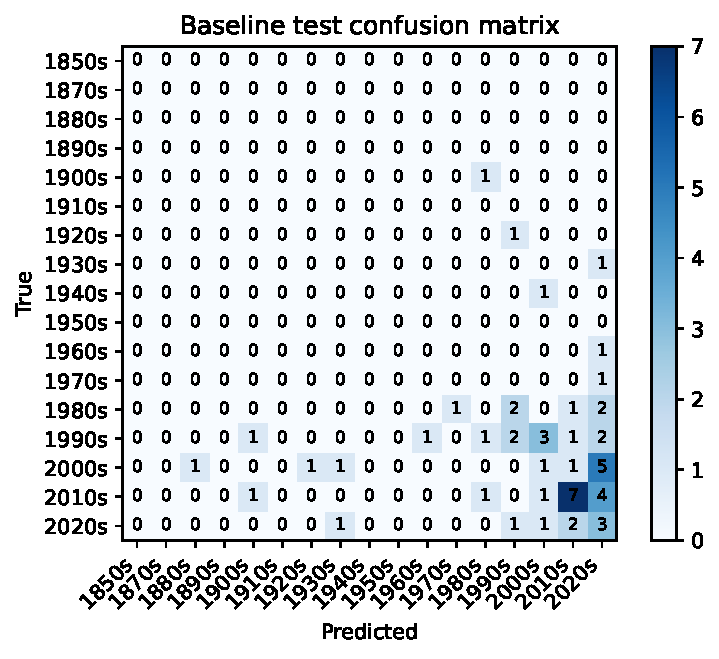
\includegraphics[width=0.46\linewidth]{figures/baseline_confusion.pdf}\hfill
  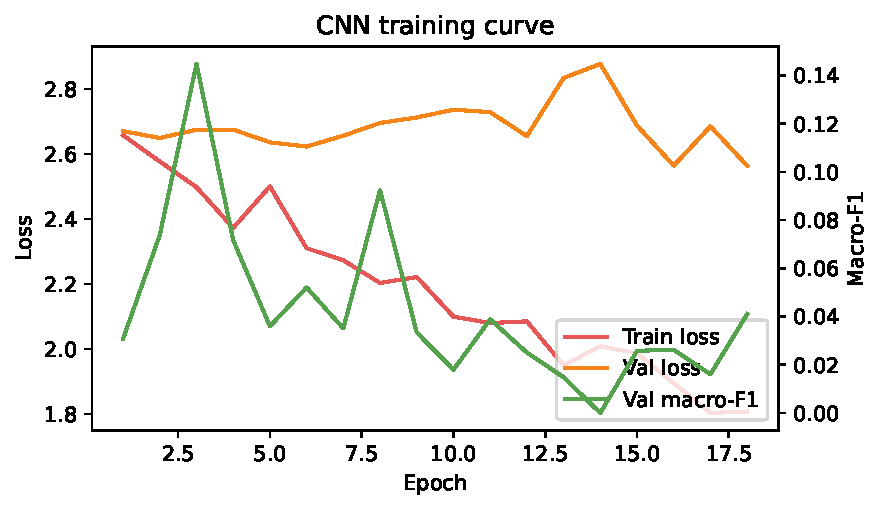
\includegraphics[width=0.46\linewidth]{figures/cnn_learning_curve.pdf}
  \caption{Left: baseline test confusion matrix. Right: CNN training curve.}
  \label{fig:models}
\end{figure}

\begin{figure}[H]
  \centering
  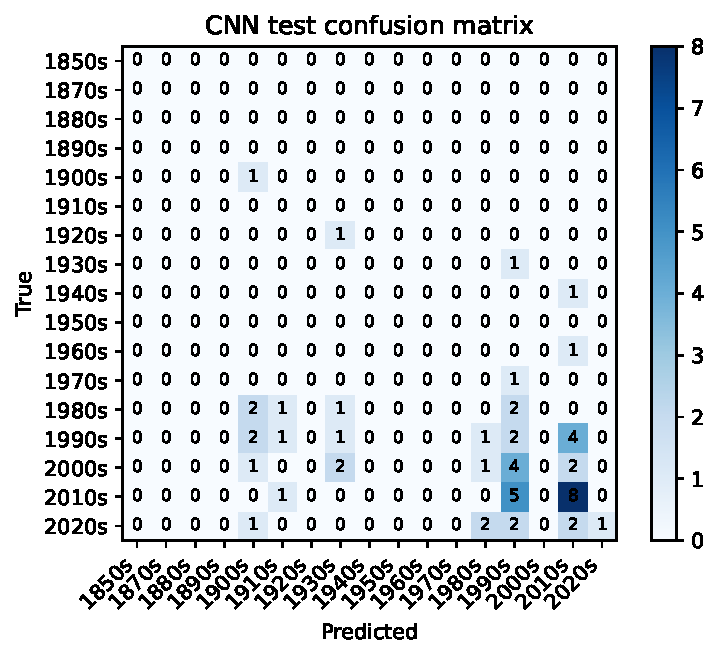
\includegraphics[width=0.55\linewidth]{figures/cnn_confusion.pdf}
  \caption{CNN test confusion matrix.}
  \label{fig:cnn_cm}
\end{figure}

\newpage

\begin{thebibliography}{99}

\bibitem{bianco2017deep}
S.~Bianco, M.~Buzzelli, D.~Mazzini, and R.~Schettini,
``Deep learning for logo recognition,''
\emph{Neurocomputing}, vol.~245, pp.~23--30, 2017.
\url{https://arxiv.org/abs/1701.02620}

\bibitem{palermo2012dating}
F.~Palermo, J.~Hays, and A.~A.~Efros,
``Dating historical color images,''
in \emph{ECCV}, pp.~499--512, 2012.
\url{https://graphics.cs.cmu.edu/projects/historicalColor/}

\bibitem{ginosar2015yearbooks}
S.~Ginosar, K.~Rakelly, S.~Sachs, B.~Yin, C.~Lee, P.~Kr\"ahenb\"uhl, and A.~A.~Efros,
``A century of portraits: A visual historical record of American high school yearbooks,''
\emph{IEEE Transactions on Computational Imaging}, 2017.
\url{https://arxiv.org/abs/1511.02575}

\end{thebibliography}

\end{document}
